
\chapter{Metodologia badań}
Niniejszy rozdział będzie opisywał kolejne etapy badań. W pierwszej kolejności wymienione zostaną narzędzia. Następnie, przedstawione będą elementy procesu eksploracji danych nie dotyczące pracy z algorytmami uczenia maszynowego, takie jak: wyszukiwanie, zbieranie, ekstrakcja cech, czyszczenie i normalizacja danych. Nawiązując do ankiety przeprowadzonej przez CrowdFlower: podczas badań związanych z {\em Big Data}, znaczącą większość czasu pochłaniana jest przez zbieranie i przygotowanie danych[link]. Zasada ta miała swoje odzwierciedlenie również w tej pracy, szczególnie, że przedmiotem badań było wideo, które wymaga wykorzystania dużych zasobów podczas tych procesów (w odróżnieniu o danych tekstowych). Na końcu opisany zostanie proces trenowania, wyniki predykcji z modeli powstałych w oparciu o algorytmy wymienione z poprzedniej sekcji.
%https://visit.figure-eight.com/rs/416-ZBE-142/images/CrowdFlower_DataScienceReport.pdf -> slajd 5
\label{cha:pierwszyDokument}

\section{Narzędzia}
Specyfika badań wymagała narzędzi będących w stanie sprawnie przetwarzać duże ilości informacji oraz zautomatyzować procesy związane z pobieraniem i przygotowaniem danych. Do tych zadań, jako optymalne rozwiązanie, został wybrany język programowania Python, według badań[link] jeden z najpopularniejszych języków programowania w {\em Data science}. Python pozwala użytkownikowi na korzystanie z zalet programowania strukturalnego, w przypadku prostych skryptów wykonujących krótkie zadanie (przykładowo: automatyczne kopiowanie i zmienianie nazw w paczkach plików), jak i obiektowego, gdzie konieczne jest ustalenie i strukturyzowanie pewnych zależności pomiędzy danymi. Dodatkową jego zaletą jest szereg bibliotek stworzonych z myślą o eksploracji danych. Do badań zostały wykorzystane następujące moduły: sklearn, pandas, selenium (framework), numpy, matplotlib.\par\par
Poniżej wymienione narzędzia posłużyły do ekstrakcji danych z plików wideo:
\begin{itemize}[label=$\bullet$]
\item ffmpg -- jest aplikacją na licencji {\em opensource} dzięki niej otrzymane zostały informacje takie jak: rozdzielczość, dane o próbkowaniu chrominancji, liczba klatek na sekundę. Dodatkowo dzięki ffmpeg skompresowane pliki wideo rozstały rozłożone na surowy format YUV.
\item {\em AGH Video Quality Indicators} -- jest ogólnodostępnym oprogramowaniem rozwijanym przez Katedrę Telekomunikacji AGH, przy jego użyciu otrzymane zostały dane o metrykach typu {\em no-reference}[link].
\item VMAF Development Kit (VDK) -- podobnie jak powyższe VDK jest ogólnodostępnym oprogramowaniem rozwijanym przez Netflix. Zaimplementowane tu zostały algorytmy liczące metryki {\em full-reference}[link].
\end{itemize}
Zbieranie danych i wydobywanie cech wideo dobywało się w dwóch środowiskach: na lokalnie działającej maszynie wirtualnej z systemem operacyjnym Xubuntu oraz na super komputerze Prometeusz[link do podziękowań czy coś w tym stylu] z systemem Centos. 

\label{cha:drugiDokument}



\section{Dane}
\label{cha:drugiDokument}

Na rysunku \ref{fig:data_preparation_work_flow} został przedstawiony schemat etapów przygotowywania danych. Aby móc pracować na dużych danych praktycznie każda z czynności dotycząca przetwarzania ich została zautomatyzowana. Kolejne akapity stanowią opis jego elementów.



\begin{center}
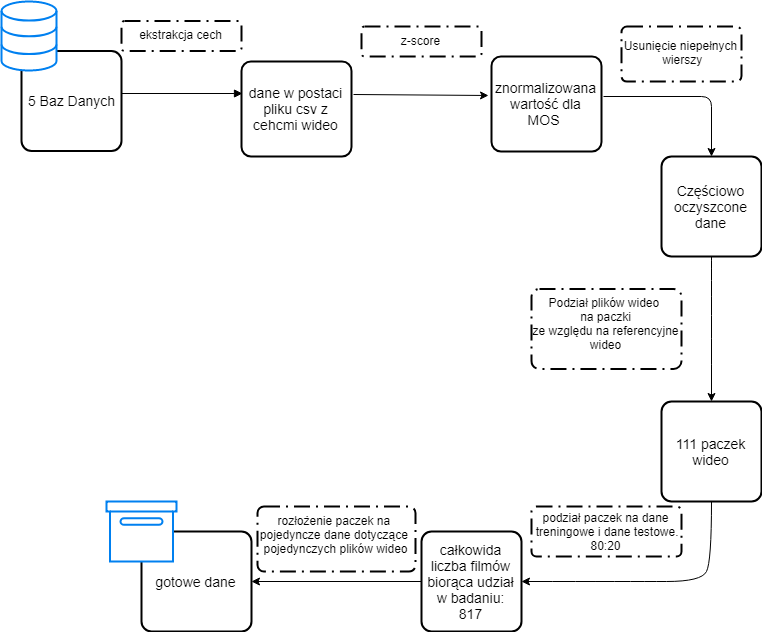
\includegraphics[ height=11cm, width=15cm]{data_preparation_work_flow}
\captionof{figure}{Schemat kroków wykonanych podczas przygotowywania danych.}
\label{fig:data_preparation_work_flow}
\label{fig:xccs}
\end{center}

\subsection{Zbieranie danych}
Aby przejść do przetwarzania danych należy je w pierwszej kolejność zebrać. Dla tego badania, podczas wyszukiwania danych, głównym kryterium było odnalezienie takich baz, gdzie oprócz plików wideo (wideo referencyjne w parze z jego zniekształconymi wersjami) istniała również jego subiektywna ocena. Ocena ludzka była konieczna, ponieważ to ona stanowiła dane nadzorcze podczas trenowania modeli. W pracy tej użyto następujące źródła danych:
\begin{itemize}
\item Subjective quality of H.264/SVC videos using ACR-HR method in VGA -- baza Danych udostępniona dzięki The Institut de Recherche en Communications et Cybernétique de Nantes. W jej skład wchodzi około 300 plików wideo ich czas trwania to: 10-12s, a rozdzielczość wszystkich wynosi: 640x480. \cite{pitrey:hal-00608310}.
\item Lab for Video and Image Analysis – LFOVIA -- jest grupą badaczy z Indian Institute of Technology Hyderabad zajmujących się tematyką jakości wideo. Dzięki udostępnionym przez nich plikom,  baza danych wejściowych w niniejszej pracy powiększyła się o 40 nowych obrazów w wysokich rozdzielczościach: FHD (1920x1080), UHD (3840x2160) i czasie trwania po 120 sekund każdy\cite{india}.
\item LIVE Netflix Video Quality of Experience Database -- baza danych stworzona przez naukowców z The University of Texas at Austin. W jej skład wchodzi 26 wideo o rozdzielczości 1920x1080, o długości 120 sekund każdy \cite{netflix_1}\cite{netflix_11}.
\item LIVE-NFLX-II Subjective Video QoE Database -- również stworzona przez The University of Texas at Austin w celu badań nad optymalnym przesyłem wideo a sieci. W bazie danych znajduje się 420 plików wideo o rozdzielczości FHD i czasie trwania około 40 sekund.
\item EPFL-PoliMI video quality assessment database -- Baza plików wideo utworzona przez dwie współpracujące uczelnie: Politecnico di Milano - Włochy i Ecole Polytechnique Fédérale de Lausanne - Szwajcaria. Dane składają się z 12 obrazów referencyjnych oraz z aplikacji pozwalającej wygenerowanie na ich podstawie zniekształconych wersji tych wideo. W ten sposób zostały uzyskane około 150 nowych filmów do badań w dwóch rozdzielczościach: 704x576, 352x288 i o czasie trwania około 10s\cite{italy}\cite{italy_2}\cite{italy_3}.
\end{itemize}
Początkowo w badaniach brała udział jeszcze jedna baza wideo z 220-oma plikami. Niestety, jak się okazało plik referencyjny oraz jego zniekształcone wersje posiadały różne wartości fps, przez co metryki typu VMAF nie były w stanie podać miarodajnych wyników. Przez co cała baza zostało pominięta.\par

\subsection{Ekstrakcja cech}
Kolejnym krokiem po zebraniu danych była ekstrakcja cech wideo, które później miały być użyte podczas przygotowywania modeli. W celu otrzymania cech każde należało wideo przekształcić do formatu surowego, nieskompresowanego YUV. Dalszy proces ekstrakcji był o tyle problematyczny, że różne, do tego wykorzystywane narzędzia, wymagały w różny sposób dostosowanych danych. Co więcej wideo bez kompresji zajmuje bardzo dużo przestrzeni dyskowej, a sam proces przetwarzania wideo wymaga również znacznego nakładu pracy dla procesora. Cechy biorące udział w badaniach to: blokowość, aktywność przestrzenna, aktywność czasowa, letterbox, pillarbox, straty bloków, rozmycie, wyciemnienie, zamrożenie, ekspozycja, kontrast, jasność, szum, PSNR, SSIM, MS-SSIM, VMAF, czas trwania, próbkowanie chrominancji, klatki na sekundę.\par
Dane dotyczące metryk $full$-$renerence$ oraz $no$-$reference$ zostały uzyskane na każdą z ramek, w następnym kroku wartości te zostały uśrednione na całe wideo. Cechy pochodzące z obu źródeł: VDK i AGH Video Quality Indicators zostały ujednolicone i zapisywanym razem w postaci pliku CSV.\par
Dodatkowo w badaniu postanowiono dodać jeszcze jedną cechę, która mogła by mieć wpływ na wynik subiektywny, to znaczy ilość różnych rozdzielczości w bazie. Przykładowo w zestawieniu, w którym pliki posiadają różne rozdzielczości, te z ich wyższą wartością (np. FHD) mogą mocniej kontrastować z tymi o niższej, przez to ocena subiektywna może okazać wyższa. W pracy jej rozpoznano dwa przypadki, kiedy baza danych zawiera pliki o jednej rozdzielczości i baza danych zawiera pliki o dwóch rozdzielczościach. Cecha ta została wprowadzona jako cecha binarna cecha nominalna dla każdego z wideo i odpowiada czy plik pochodzi z bazy o jednej rozdzielczości. Jeżeli tak to wartość jej przyjmuje 1, w innym wypadku 0. [edit] jest to czynnik ktory bylo by ciezko ogarnąć w praktycznym zastosowaniu, w badaniu może być. W praktyce musiało by to oznaczac ze wiemy jaki zbiór filmów użytkownik oglądał wcześniej.[edit] \par
Jako cechę nadzorującą użyto subiektywną ocenę ludzką.\par

\subsection{Normalizacja i czyszczenie danych}
W zbiorze plików pochodzących do badaczy z uniwersytety w Texas-ie ocena subiektywna została przekazana po znormalizowaniu $z$-$score$, gdzie zakres wartości zawiera się pomiędzy -3, a 3. W celu otrzymania miarodajnych wyników dane z pozostałych baz również zostały w ten sam sposób znormalizowane.\par
Podczas procesu przygotowywania danych jaki i późniejszej ekstrakcji cech mogły nastąpić pewne wyjątki, które uniemożliwiły otrzymanie poprawnego wyniku. W takim przypadku cały wiersz dotyczący danego wideo był pomijany podczas tworzenia modeli.

\subsection{Przygotowanie formatu danych pod modelowanie}

Przy tworzeniu modeli została wykorzystana implementacja zawarta w module języka Python sklearn. Instancję klas przedstawiających algorytmy przyjmują jako dane wejściowe dane w formacie macierzy. Dlatego pliki CSV zostały, podczas działania skryptu, przekształcone do typu DataFarme. Wspierany jest on przez moduł, ułatwiający prace z danymi, pandas.\par

Przy eksploatowaniu danych często stosuje techniką jest $ang.$ $cross$ $validation$. Polega ona na podziale na dostępnych przy badaniu danych na dane treningowe i testowe. Można tu wykorzystać zasadę podziału 80:20, co oznacza ze 80 części danych jest przeznaczonych na dane treningowe, a 20 na dane testujące. Dobrym podejściem jest, aby w obu z tych grup znalazły się dane z całego przekroju bazy danych. Skutkuje to ograniczeniem problemu generalizacji czy nad dopasowania. W niniejszej pracy proces podziału danych należało przeprowadzić, tak aby uwzględnić "paczki" danych, czyli wideo referencyjne oraz jego zniekształcenia. Dane z jednej paczki powinny w całości znaleźć się w grupie danych testowych bądź treningowych. Schemat podziału jest przedstawiony na rysunku \ref{fig:podzial_danych}.
\begin{center}
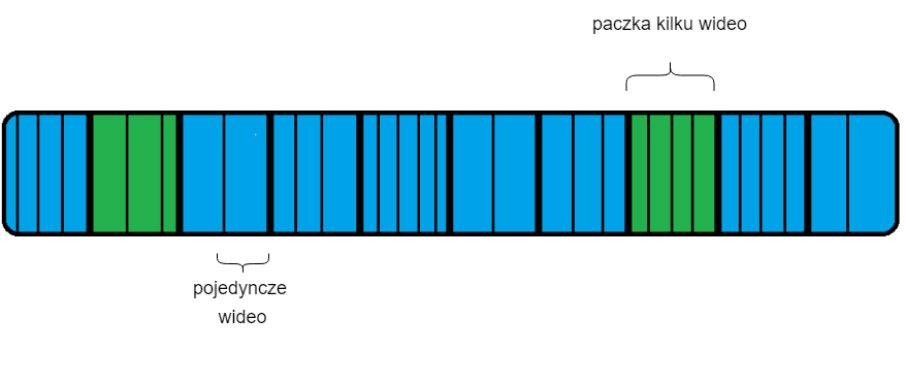
\includegraphics[ height=5cm, width=10cm]{podzial_danych}
\captionof{figure}{Przykładowy podział danych na dane testowe i treningowe (80:20). Niebieskie prostokąty odnoszą się do danych treningowych, a zielone do danych testowych.}
\label{fig:podzial_danych}
\label{fig:xccs}
\end{center}
Ostatnim etapem podczas przygotowywania danych było połączanie danych z każdej paczki. Od tego momentu wektor danych wejściowych podczas przygotowywania modelu odnosi się do pojedynczego pliku wideo.




\subsection{Podsumowanie danych}
Poniższa tabela \ref{tab:tabela} przedstawia uzyskane dane 


\begin{table}[!htbp]
\centering
\begin{tabular}{|c|l|l|l|l|}
\hline
\multicolumn{5}{|c|}{5 baz danych, ponad 800 wektorów danych, ponad 100 paczek plików wideo} \\ \hline
\multicolumn{5}{|c|}{21 cech statystycznych} \\ \hline
\multicolumn{2}{|c|}{ilościowe} & \multicolumn{3}{c|}{jakościowe} \\ \hline
\multicolumn{2}{|l|}{\begin{tabular}[c]{@{}l@{}}blokowość, aktywność przestrzenna, aktywność czasowa,\\ letterbox, pillarbox, straty bloków, rozmycie, wyciemnienie, \\ zamrożenie, ekspozycja, kontrast, jasność, szum, \\ PSNR, SSIM, MS-SSIM, VMAF, czas trwania,\end{tabular}} & \multicolumn{3}{l|}{\begin{tabular}[c]{@{}l@{}}próbkowanie chrominancji,\\ rozdzielczość, \\ ilość dostępnych rozdzielczości\end{tabular}} \\ \hline
\end{tabular}
\caption{Podsumowanie przygotowania danych}
\label{tab:tabela}
\end{table}

Dodatkowo analizując dane można wyszczególnić korelację pomiędzy poszczególnymi cechami : 



\section{Modele }
\label{cha:drugiDokument}
W niniejszej pracy zostały przetestowane cztery algorytmy uczenia maszynowego przedstawione w części teoretycznej. Parametry definiujące ich działanie zostały dobra na zasadzie obserwacji i wiedzy na temat ich działania.\par

Regresja liniowa została sprawdzona w pierwszej kolejności. Jako jeden prostszych z algorytmów, nie jest tu wymagane podawanie dodatkowych parametrów, aby algorytm zadziałał w prawidłowy sposób. W tym przypadku wektor danych wejściowych podczas trenowania wygląda następująco: $y_i = \beta_0 + \beta_1 x_{1i} + \beta_2 x_{2i} + ... + \beta_p x+x_{pi} + \epsilon $, gdzie $y_i$ jest subiektywną oceną dla filmu $i$, a $x_{1i}, x_{2i}...$ są jego cechami. \par

Kolejnym testowanym algorytmem był SVR. Użyta funkcja kernela do wyznaczenia hiperpłaszczyzny to $Radial$ $Basis$ $Function$ (RBF). Współczynnikowi $\epsilon$ została przypisana wartość $0,1$. $\gamma$, która mówi jak odległe punkty będą miały wpływ na budowaną hiperpłaszczyznę, otrzymała wartość $auto$, a parametr $C$, który odpowiada za gładkość funkcji SVR wynosi 0.7.\par
%https://www.ncbi.nlm.nih.gov/pmc/articles/PMC2839056/

Random Forest działa w oparciu o parametry podane przez badacza, takie jakie jak ilość drzew i ich głębokość. W tym przypadku użyto 100 drzew o głębokości 8. Jako metodę podziału danych , podczas budowy drzewa regresyjnego , zostały wybrany:xx\par

Ostatnim sprawdzonym algorytmem uczenia maszynowego była sieć neuronowa z następującymi parametrami: 3 warstw ukrytych po 13 neuronów w każdej. Maksymalna ilość iteracji algorytmu $Backward$ $Propagation$ po której model będzie gotowy to 1000. Parametr $learning$ $rate$, określający szybkość uczenia, został ustawiony na wartość 0,001.\par

Z uwagi na specyfikę przygotowania danych treningowych i testowych każdy z modeli został zbudowany i przetestowany x razy. Podział danych 80:20 dotyczy paczek wideo, natomiast budowa modeli odbywa się już na podstawie pojedynczych plików wideo. Dlatego może zaistnieć sytuacja kiedy większość małych paczek (np. po 3 pliki wideo) znajdą się w danych treningowych, a duże (np. po 15 wideo) w danych testujących. Tym samym faktyczny podział może wynosić w skrajnym przypadku 50:50, zamiast 80:20 (taki sam odstęp może wystąpić w drugą stronę). Dlatego przy uruchomieniu każdej z symulacji (użycie każdego z algorytmów) podział danych dobywał się na zasadzie losowo wybranych paczek do każdej grup, przy zachowaniu podziału 80:20. Następnie wyniki z przeprowadzonych uruchomień programu zostały uśrednione.\par
W ramach kolejnych prób modele były budowane i testowane na następujących zestawach cech wideo:
\begin{enumerate}
\itemsep-0.5em 
\item VMAF
\item VMAF, SSIM
\item MS-SSIM
\item PSNR
\item PSNR, VMAF
\item PSNR, VMAF, SSIM, MS-SSIM, blokowość
\item PSNR, VMAF, SSIM, MS-SSIM, blokowość, rozdzielczość
\item PSNR, VMAF, SSIM, MS-SSIM, blokowość, jasność, ilość dostępnych rozdzielczości
\item PSNR, VMAF, SSIM, MS-SSIM, blokowość, jasność, ilość dostępnych rozdzielczości, rozdzielczość
\item PSNR, VMAF, SSIM, MS-SSIM, blokowość, aktywność przestrzenna, pillarbox, straty bloków, rozmycie, aktywność czasowa, zaciemnienie, ekspozycja, kotrast, jasność, czas trwania, rozdzielczość
\item PSNR, VMAF, SSIM, MS-SSIM, blokowość, aktywność przestrzenna, pillarbox, straty bloków, rozmycie, aktywność czasowa, zaciemnienie, ekspozycja, kotrast, jasność, ilość dostępnych rozdzielczości, czas trwania, rozdzielczość
\item PSNR, VMAF, SSIM, MS-SSIM, czas trwania
\item PSNR, VMAF, SSIM, MS-SSIM, czas trwania, rozdzielczość
\item PSNR, VMAF, SSIM, MS-SSIM, czas trwania, blokowość, jasność, ilość dostępnych rozdzielczości
\item PSNR, VMAF, SSIM, MS-SSIM, czas trwania, blokowość, jasność, ilość dostępnych rozdzielczości, rozdzielczość
\item PSNR, VMAF, SSIM, MS-SSIM, czas trwania, jasność, blokowość
\item PSNR, VMAF, SSIM, MS-SSIM, czas trwania, jasność, blokowość, rozdzielczość
\item PSNR, VMAF, SSIM, MS-SSIM, czas trwania, ilość dostępnych rozdzielczości
\item PSNR, VMAF, SSIM, MS-SSIM, czas trwania, ilość dostępnych rozdzielczości, rozdzielczość
\item PSNR, SSIM
\item SSIM
\item blokowość,
\item blokowość, aktywność przestrzenna, pillarbox, straty bloków, rozmycie, aktywność czasowa, zaciemnienie, ekspozycja, kotrast, jasność, czas trwania, ilość dostępnych rozdzielczości, rozdzielczość
\item blokowość, aktywność przestrzenna, pillarbox, straty bloków, rozmycie, aktywność czasowa, zaciemnienie, ekspozycja, kotrast, jasność, czas trwania, rozdzielczość
\item jasność,
\item kotrast,
\item czas trwania,
\item ekspozycja,
\end{enumerate}

Dalsze rozdziały będą odnosić się do powyższej numeracji w kontekście zestawów cech.


\chapter{Wyniki i analiza }
Poniższy rozdział, w pierwszej kolejności,  zaprezentuje wyniki  z poszczególnych modeli. Zostały one zebrane na wykresach słupkowych, gdzie os x odnosi się do numerów zestawów, a os y do średnich wartości R-kwadrat \ref{fig:podsumowanie}. W dalszej części rozdziału  odbędzie się ich analiza.


\begin{sidewaysfigure}[ht]
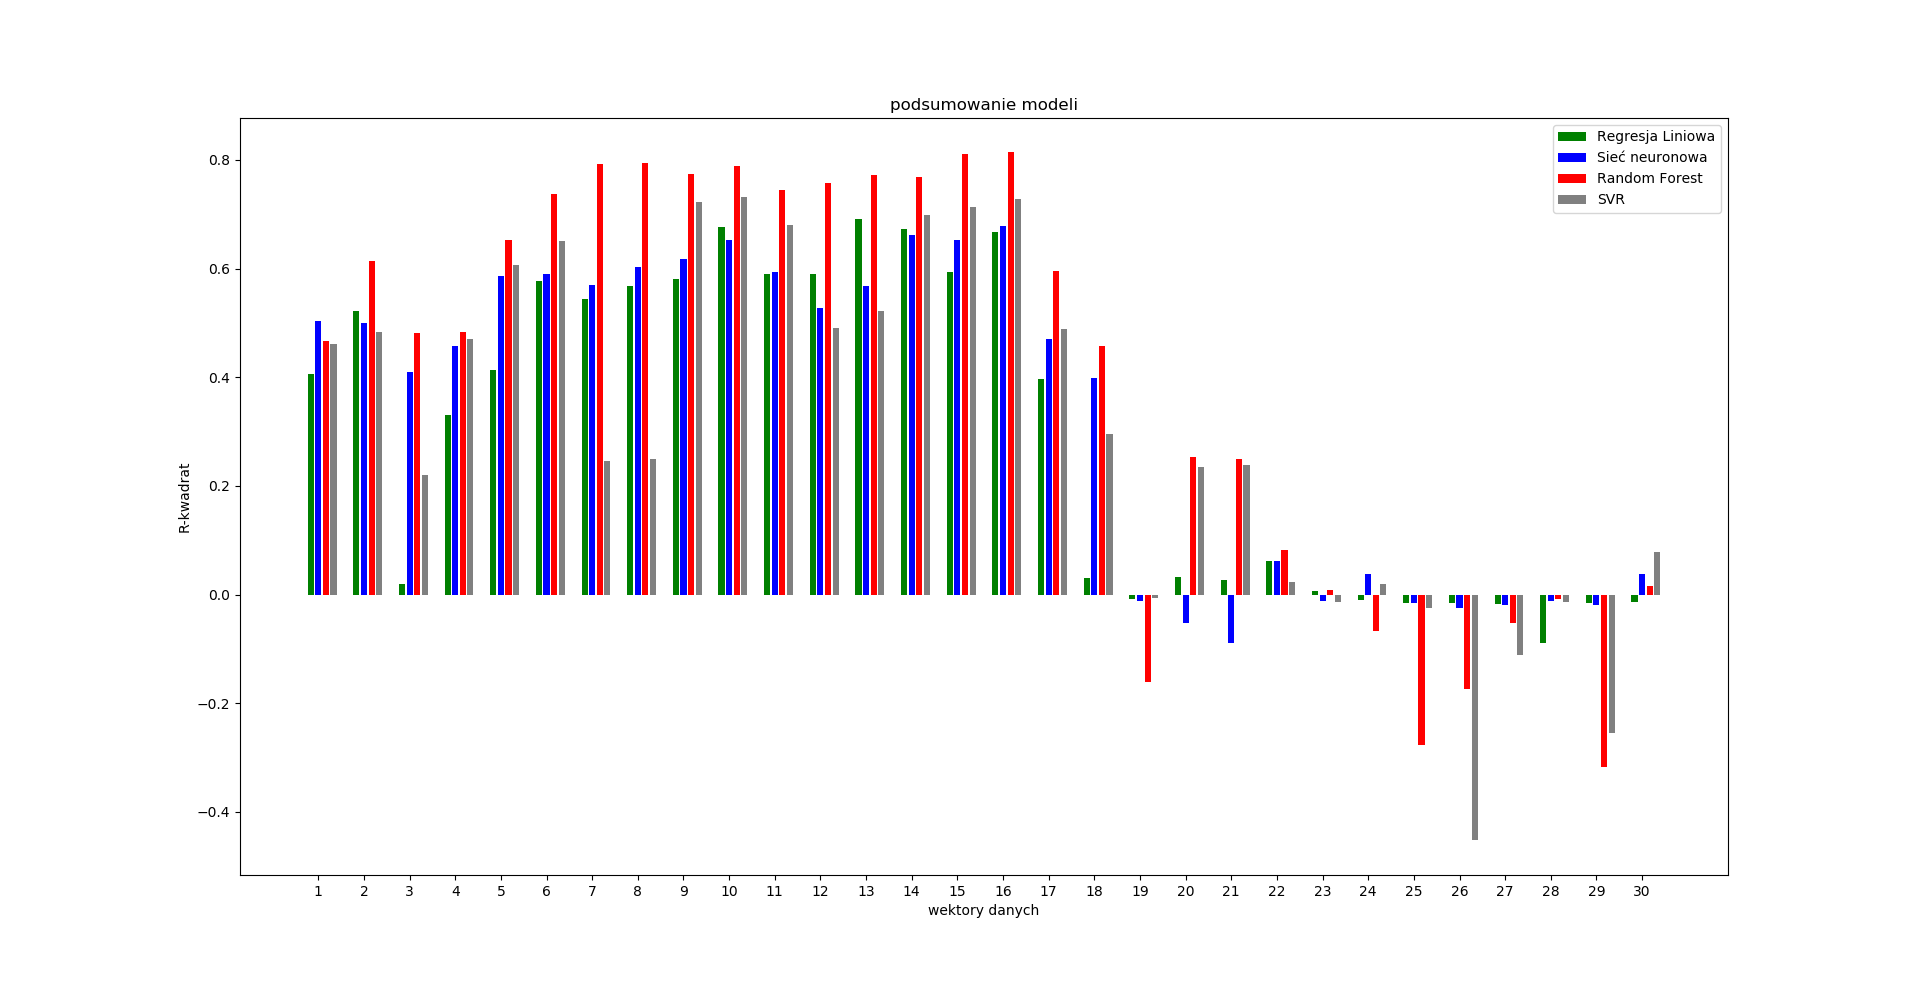
\includegraphics[ height=15cm, width=26cm]{podsumowanie}
\captionof{figure}{Wyniki z poszczególnych modeli}
\label{fig:podsumowanie}
\label{fig:xccs}
\end{sidewaysfigure}

W pierwszej kolejności wyjaśniane zostaną różnice w obrębie zestawów danych, a pomiędzy poszczególnymi modelami.  Wynikać to może z charakterystyki testowanych algorytmów uczenia maszynowego. Niektóre z nich potrafią odnaleźć fałszywe zależności w danych testowych, które nie wystąpiły w czasie testów, czyli występuje  nad-dopasowanie dla pewnych cech. Inna przyczyną możne być generalizacja, przez którą może nastąpić pominięcie pewnych informacji ukrytych w danych.\par

Obserwując poszczególne wyniki dla zestawów $no$-$reference$ (1 -- 12)  oraz $full$-$reference$ (13 -- 20, 29, 30) można zaobserwować, że te drugie znacznie trafniej dokonują predykcji. Może to wynikać z tego , że metryki  $no$-$reference$ wymagają stworzenia osobnych modeli  z innymi parametrami. Co  więcej algorytm wykazał że wprowadzona dodatkowa cecha (ilość dostępnych rozdzielczości) , choć w niewielkim stopniu, również ma  wpływ na ocenę jakość. W większości przypadków zestaw z tą cecha otrzymywał wyższe R-kwadrat, niż ten sam ale bez niej. Przykłady tej zależności przedstawione są w tabeli \ref{tab:tabela rozdzielczosc}. Podobne, sprawdzone tu, oddziaływanie to czas trwania. Dla dłuższych wideo  model daje lepsze wyniki, różnice również są nieznaczne. \par

\begin{center}
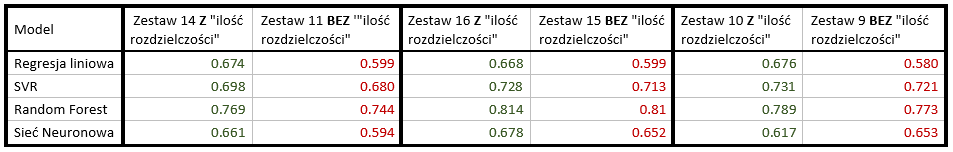
\includegraphics[ height=4cm, width=17cm]{tabela_rozdzielczosc}
\captionof{figure}{zestawy (11, 14), (9,10), (15, 16) są dla siebie bliźniacze z różnicą dodatkowej cechy.}
\label{tab:tabela rozdzielczosc}
\label{fig:xccs}
\end{center}
  
Na wykresie \ref{fig:podsumowanie} można dostrzec, że różnice pomiędzy nim kilkoma  zastawem jest niewielka, przy większości modeli. Dla tych zestawów wspólnym mianownikiem są cechy: PSNR, VMAF, SSIM, MS-SSIM. Każda z cech również osiąga wysokie wyniki (R-kwadrat kolejno dla modelu Lasu Losowego: 0.484, 0.467, 0.458,  0.481), niższe jednak niż te osiągnięte w zestawie.  Co więcej wymienione wyżej cechy posiadają wysoki współczynnik korelacji \ref{fig:korelacja}, przez co łączenie ich tylko w pewnym stopniu poprawia trafność modelu, końcowa wartość nie jest ich sumą. Przykładowo dla zestawu 2 (VMAF + SSIM) R-kwadrat wynosi 0.614 \par



\begin{center}
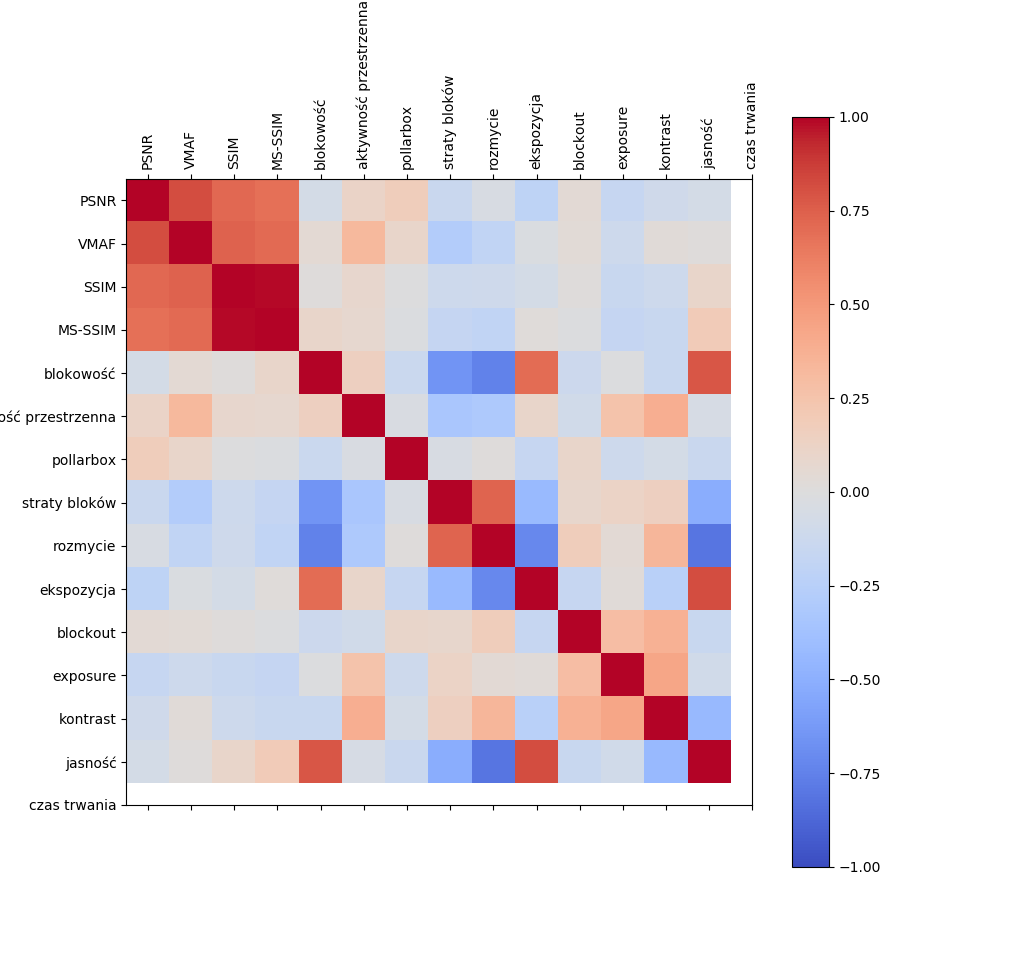
\includegraphics[ height=14cm, width=14cm]{korelacja}
\captionof{figure}{Korelacja pomiędzy PSNR, SSIM, MS-SSIM, VMAF}
\label{fig:korelacja}
\label{fig:xccs}
\end{center}





Kolejny aspekt, który można odnotować czytając wykres to ujemna wartość R-kwadrat dla niektórych zestawów. Biorąc pod uwagę wzór \ref{eqn:r2}, oznacza to , że model podczas testów dokonywał gorszej predykcji, niż średnia dla zbioru danych testowych. Tą sytuację przedstawia wykres \ref{fig:kontrast_ujemne_rk}. Zaprezentowane są tu próbki danych dla cechy kontrast. Funkcja regresji liniowej (linia niebieska)  pokrywa się ze średnią dla danych testowych (linia pomarańczowa), ale podczas liczenia R-kwadrat brana pod uwagę jest średnia ze zbioru danych testowych (linia czerwona). Gdy by ta ostania pokrywała się z linią regresji R-kwadrat wynosił by 0. Ujemny R-kwadrat oznacza również, że dla danej cechy lub ich zestawu, algorytm nie odnalazł zależności miedzy zmiennymi opisującymi, a zmienną opisywaną.\par
\begin{center}
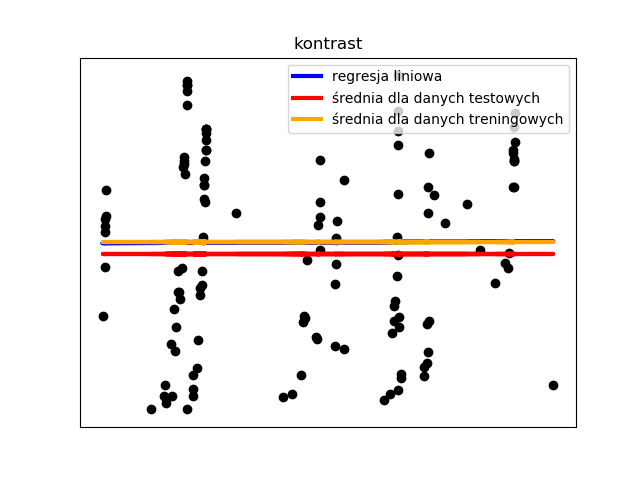
\includegraphics[ height=9cm, width=13cm]{kontrast_ujemne_rk}
\captionof{figure}{Przypadek kiedy wskaźnik r-kwadrat jest ujemny.}
\label{fig:kontrast_ujemne_rk}
\label{fig:xccs}
\end{center}

Najwyższy uśredniony wynik R-kwadrat został osiągnięty przez model zbudowany na podstawie algorytmu Lasu Losowego(z zadanymi wcześniej parametrami) z użyciem zestawu 16, czyli 0.814. Składa się on z  zebranych metryk full-reference z uwzględnieniem czasu trwania wideo i dodatkowej cechy dotyczącej ilości dostępnych rozdzielczości. Odnosząc się do tematu pracy, ma on największą szanse na trafne wyznaczenie jakość wideo. Konkretny model nie jest tu odpowiedzią ponieważ bazuje się tu na podstawie uśrednionych wyników z ponad 100 wykonań programu. Każdy z modeli z tej grupy z daje różne wyniki (odchylenie standardowe wynosi 0.053 i jest stosunkowo nieduże w porównaniu z innymi modelami i zestawami) ponieważ budowany jest na różnych próbkach danych.  \par




\chapter{Podsumowanie}


Założeniem niniejszej pracy było stworzenie algorytmu oceniającego jakość wideo. Po uprzednim przygotowaniu do dyspozycji podczas badań były  informacje opisujące wideo, zarówno metryki FR i NR. Zostaly one wykorzystane do przystosowania i zbudowania 4 modeli w oparciu o algorytmy uczenia maszynowego. 
To wytrenowane modele mogą posłużyć jako algorytm oceniający jakość wideo. W niniejszej pracy jako zbudowano odpowiedni ponad 100 modeli dla każdego z algorytmów, aby zniwelować  różnice wynikające z specyficznego podziału danych. Dlatego wynikiem badań nie jest  jeden konkretny model, a "przepis" jak go otrzymać.\par

Nie można powiedzieć, że rozwiązanie tu przedstawione będzie uniwersalnym wyznacznikiem jakości wideo. Możliwe, że istnieją inne czynniki, które nie zostały uwzględnione. Badanie to korzysta z oceny ludzkiej jako z cechy nadzorującej, z tego faktu mogą wynikać nie brane pod uwagę efekty zmieniające tą ocenę. Przykładowo z biegiem lat oczekiwania co do jakości mogą znacznie się zmienić. Taką tendencję można zaobserwować porównując typowe wideo z lat 90, wtedy uważane za wysokiej klasy i współczesne wideo. Dalej rozważając,  bazując na metrykach FR to mimo że wszystkie one mają wysokie wartości, to jeżeli wideo referencyjne jest już na samym początku zniekształcone to wizualna ocena widza też będzie negatywna. \par

Przedstawione w tej pracy rozwiązanie, jak również zebrane dane mogą posłużyć przy dalszych badaniach nad wideo. W rozwinięciu pracy  można uwzględnić nowe cechy. Na przykład w podobny sposób stworzonej tu "ilość dostępnych rozdzielczości w bazie". Innym bardziej zaawansowanym podejściem było by stworzenie metryki, która była by  w stanie na bieżącą dostosowywać się i oceniać wideo, w zależności od aktualnego rodzaju zniekształcenia obrazu.\par



ulepsznie: poprzez zróznicowanie wag podczas trenowania
wyniki nie koniecznie sa miarodajne, poniwaz występpowanie róznych cech nie oniecznie bylo zrównoważone
dasuidhkasudhkajshdk
\label{cha:pierwszyDokument}









